\documentclass[a4paper]{article}

\usepackage{amsmath}
\usepackage{CJKutf8}
\usepackage{indentfirst}
\setlength{\parindent}{2em}
\usepackage{listings} %插入代码
\usepackage{xcolor} %代码高亮
\lstset{numbers=left, %设置行号位置
        %numberstyle=\tiny, %设置行号大小
        %keywordstyle=\color{blue}, %设置关键字颜色
        %commentstyle=\color[cmyk]{1,0,1,0}, %设置注释颜色
        frame=single, %设置边框格式
        escapeinside=``, %逃逸字符(1左面的键),用于显示中文
        breaklines, %自动折行
        extendedchars=false, %解决代码跨页时,章节标题,页眉等汉字不显示的问题
        xleftmargin=2em,xrightmargin=1em, aboveskip=1em, %设置边距
        tabsize=4, %设置tab空格数
        showspaces=false %不显示空格
        }
\usepackage{graphicx} 

\renewcommand{\contentsname}{目录}
\renewcommand{\listfigurename}{插图目录}
\renewcommand{\listtablename}{表格目录}
\renewcommand{\refname}{参考文献}
\renewcommand{\abstractname}{摘要}
\renewcommand{\indexname}{索引}
\renewcommand{\tablename}{表}
\renewcommand{\figurename}{图}

\title{数据结构基础讲义}
\author{哈尔滨工程大学ACM集训队}
\date{\today}

\begin{document}
\begin{CJK}{UTF8}{gbsn}
\maketitle
\newpage

\tableofcontents
\newpage
\begin{abstract}
\begin{CJK}{UTF8}{gkai}
算法是指为了达到某种目的而操作数据的方式。算法通常适用于具体的问题,以复杂的方式来处理简单的数据。例如,编译器把简单的字符串和字符翻译成可以在特定机器上执行的二进制代码。编译器内部的工作原理是:通过相互影响的诸多算法按顺序将源代码字符转换为中间表示。这些表示都是通过其他算法将他们自身翻译成目标代码,这些代码与原始的字符和字符串具有极少的相似之处。尽管程序不像编译器那样有雄心壮志,但它们也同样极大地依赖于算法,以一种可预见的方式来处理数据。因此,在不了解操作数据的基本例程的情况下,不可能深入地讨论算法。那些希望通晓如何使用算法的开发人员首先要学习如何操作数据。而后,它们可以根据自己的需要应用算法技术来表示数据。\cite{pap}

我们将讨论数据结构中最简单的内容,即线性表和树形结构,并增加一些补充内容。
\end{CJK}
\end{abstract}

\section{线性结构}
线性表是最基本、最简单、也是最常用的一种数据结构。线性表中数据元素之间的关系是一对一的关系,即除了第一个和最后一个数据元素之外,其它数据元素都是首尾相接的。线性表的逻辑结构简单,便于实现和操作。因此,线性表这种数据结构在实际应用中是广泛采用的一种数据结构。线性表的特征可以由一下几点概括:
\begin{enumerate}
\item 存在唯一的一个被称做“最后一个”的数据元素;
\item 除第一个之外,每个元素都只有一个前驱;
\item 除最后一个之外,每个元素都只有一个前驱;
\item 除最后一个之外,每个元素都只有一个后继。
\end{enumerate}
在这里我们只讨论几个简单的线性结构,并在最后探讨他们的应用。

\subsection{数组}
数组应该是线性表中使用次数最多的数据结构, 而且数组的实现使得命令式语言中抽象数据结构的实现成为可能。

\subsubsection*{认识数组}
数组是电脑编程语言上,对于“Array”的中文称呼。它十分类似数学上的“矩阵”, 但是在电脑编程语言上,表示方法和意义上略有不同。\\
数学上的矩阵看起来像这样:
$$
a=
\begin{bmatrix}
4&9&2\\
3&5&7\\
8&1&6
\end{bmatrix}
$$
而电脑上的数组看起来像这样,例如C语言\footnote{今后若无特别说明,所用代码均为C/C++。} 中的数组:
\begin{lstlisting}[language=C]
int a[3][3]={ 
            { 4,  9,  2 },
            { 3,  5,  7 },
            { 8,  1,  6 }
};
\end{lstlisting}

我们可以把数组当成一个向量\footnote{相信线性代数老师已经强调过向量的概念了。}。比如上面的数组a,令$a_1$,$a_2$,$a_3$为包含3个整数的向量:
$a1=\begin{bmatrix}4&9&2\end{bmatrix}, a2=\begin{bmatrix}3&5&7\end{bmatrix}, a3=\begin{bmatrix}8&1&6\end{bmatrix}$,则a为一个包含$a_1$,$a_2$,$a_3$的向量:

$$
a=
\begin{bmatrix}
a_1&a_2&a_3
\end{bmatrix}
$$

当然,你也可以仅将一维数组当成一个向量,而把二维数组当成一个矩阵,再把三维数组当成一个立方体。但我相信,过一段时间之后,你会坚持我们前面所说的模型的。

\subsubsection*{C/C++中的数组}
这么说可能会让你不舒服,但是C语言并不支持数组这种数据类型,至少不像整形,浮点型甚至结构体那样支持数组。C/C++使用一种奇怪的方式来实现数组,这导致了理解上的麻烦。

我们定义数组时使用的格式如下:

\begin{center}
类型名 数组名 [数组长度]
\end{center}
例如
\begin{lstlisting}[language=C++]
int A[10];
float b[10], c[20];
char ch[20];
\end{lstlisting}
第1行说明整型数组a,有10个元素;
第2行说明实型数组b,有10个元素,实型数组c,有20个元素;
第3行说明字符数组ch,有20个元素。

数组长度和类型名同属这个数组的类型,但一个在数组名的前面,另一个在数组名的后面,这是比较容易混淆的地方。当我们定义一个如上文中提到的二维数组a时,最后的方括号表示的不是向量a的长度,而是它所包含的每个向量长度即$a_1$,$a_2$,$a_3$的长度。数组的长度紧跟着数组名,而之后的方括号说明的是这个数组所包含的元素的类型。

我们可以通过下标或指针来使用数组中的元素:

\begin{lstlisting}[language=C++]
// using_arrays.cpp
int main() {
   char chArray[10];
   char *pch = chArray;   // Evaluates to a pointer to the first element.
   char   ch = chArray[0];   // Evaluates to the value of the first element.
   ch = chArray[3];   // Evaluates to the value of the fourth element.
}
\end{lstlisting}

当数组名和指针混用时,我们应该注意它们之间的区别。除了 sizeof 运算符和 \& 运算符后面出现的数组名之外,数组名都被当做一个指针常量。在上面的程序中,pch 和 chArray 在大多数情况下是等价的,可以像使用数组名一样使用 pch。数组名当做函数的参数时,它被当做一个指针,这时函数内的数组就是这个数组,而不是一个它的拷贝,在函数内改变这个数组和在函数外改变这个数组是一样的。

如果想使用长度不确定的数组,或者想把数组存入堆区而非栈区,可以使用下面的方法:

\begin{lstlisting}[language=C++]
#define ARRAY_SIZE
/****C****/
#include <malloc.h>
int *p = malloc(sizeof(int) * ARRAY_SIZE);
//use array here
free(p); //must free it after used!

/****C++****/
int *q = new int[ARRAY_SIZE];
//use array here
delete[] q; //must delete it after used!
\end{lstlisting}

这里附上几天之前提到过的快速排序算法。
\begin{lstlisting}[language=C++]
void quickSort(int arr[], int left, int right) {
      int i = left, j = right;
      int tmp;
      int pivot = arr[(left + right) / 2];
 
      /* partition */
      while (i <= j) {
            while (arr[i] < pivot)
                  i++;
            while (arr[j] > pivot)
                  j--;
            if (i <= j) {
                  tmp = arr[i];
                  arr[i] = arr[j];
                  arr[j] = tmp;
                  i++;
                  j--;
            }
      };
 
      /* recursion */
      if (left < j)
            quickSort(arr, left, j);
      if (i < right)
            quickSort(arr, i, right);
}
\end{lstlisting}

\subsubsection*{更像向量的数组}

在C++中,我们可以使用一个更像向量的数据类型。之所以说''更像''是因为名字就像\raisebox{0.1em}{------}这种类型叫做vector。它是一个可变长的数组。\footnote{更详细的用法可以RTFM。}
\begin{lstlisting}[language=C++]
vector< int > line
for(int i = 0 ; i < 10 ; i ++) {
    line.push_back(line);
}
for(int i = 0 ; i < 10 ; i ++) {
    cout << line[i] << endl;
}
\end{lstlisting}

\subsection{栈和队列}
栈和队列都是动态集合,且在其上进行DELETE操作所移除的元素是预先设定的。在栈(stack)中,被删除的是最近插入的元素:栈实现的是一种后进先出的(last-in,first-out,LIFO)策略。类似地,在队列(queue)中,被删去的总是在集合中存在时间最长的那个元素:队列实现的是一种先进先出(first-in,first-out,FIFO)策略。在计算机上实现栈和队列有几种有效方式。我们将介绍如何利用一个简单的数组实现这两种结构。
\subsubsection*{栈}
栈上的INSERT操作称为PUSH,而DELETE操作称为POP,这两个名称使人想到现实中的栈,比如餐馆里装有弹簧的摞盘子的栈。盘子从栈中滑出的次序刚好同他们压入的次序相反,这是因为只有最上面的盘子才能被取下来。

如下图所示,可以用一个数组$S[1..n]$来表示一个最多可容纳$n$个元素的栈。该数组有一个属性$S.top$,指向最新插入的元素。栈中包含的元素为$S[1..S.top]$,其中$S[1]$是栈底元素,而$S[S.top]$是栈顶元素。

\begin{figure}[htbp]
\centering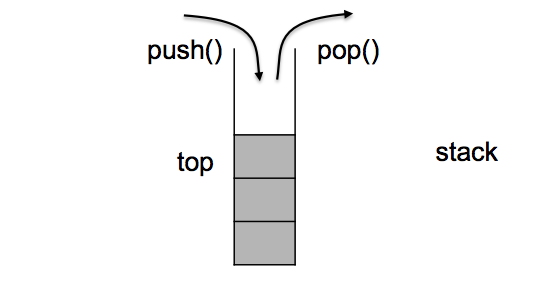
\includegraphics[height=3cm]{stack1.png}
\caption{栈的结构}
\end{figure}

\begin{lstlisting}[language=C]
/*
** A stack implemented with a static array.  The array size can
** be adjusted only by changing the #define and recompiling
** the module.
*/
#include "stack.h"
#include <assert.h>

#define	STACK_SIZE	100	/* Max # of values on the stack */

/*
**	The array that holds the values on the stack, and a pointer
**	to the topmost value on the stack.
*/
static	STACK_TYPE	stack[ STACK_SIZE ];
static	int		top_element = -1;

/*
**	push
*/
void
push( STACK_TYPE value )
{
	assert( !is_full() );
	top_element += 1;
	stack[ top_element ] = value;
}

/*
**	pop
*/
void
pop( void )
{
	assert( !is_empty() );
	top_element -= 1;
}

/*
**	top
*/
STACK_TYPE top( void )
{
	assert( !is_empty() );
	return stack[ top_element ];
}

/*
**	is_empty
*/
int
is_empty( void )
{
	return top_element == -1;
}

/*
**	is_full
*/
int
is_full( void )
{
	return top_element == STACK_SIZE - 1;
}
\end{lstlisting}

栈的实现方法当然不会只有一种,也不会只有两种。下面给出栈的链表(see below)实现。

\begin{lstlisting}[language=C]
/*
** A stack implemented with a linked list.  This stack has no size
** limit.
*/
#include "stack.h"
#include <stdio.h>
#include <stdlib.h>
#include <malloc.h>
#include <assert.h>

#define	FALSE 0

/*
**	Define a structure to hold one value.  The link field will
**	point to the next value on the stack.
*/
typedef	struct	STACK_NODE {
	STACK_TYPE	value;
	struct STACK_NODE *next;
} StackNode;

/*
**	A pointer to the topmost node on the stack.
*/
static	StackNode	*stack;

/*
**	create_stack
*/
void
create_stack( size_t size )
{
}

/*
**	destroy_stack
*/
void
destroy_stack( void )
{
	while( !is_empty() )
		pop();
}

/*
**	push
*/
void
push( STACK_TYPE value )
{
	StackNode	*new_node;

	new_node = malloc( sizeof( StackNode ) );
	assert( new_node != NULL );
	new_node->value = value;
	new_node->next = stack;
	stack = new_node;
}

/*
**	pop
*/
void
pop( void )
{
	StackNode	*first_node;

	assert( !is_empty() );
	first_node = stack;
	stack = first_node->next;
	free( first_node );
}

/*
**	top
*/
STACK_TYPE top( void )
{
	assert( !is_empty() );
	return stack->value;
}

/*
**	is_empty
*/
int
is_empty( void )
{
	return stack == NULL;
}

/*
**	is_full
*/
int
is_full( void )
{
	return FALSE;
}
\end{lstlisting}


\subsubsection*{队列}
队列上的INSERT操作称为ENQUEEUE,DELETE操作称为DEQUEUE;正如栈的POP操作一样,DEQUEUE操作也没有元素参数。队列的先进先出特性类似于收银台前排队等待结账的一排顾客。队列有队头(head)和队尾(tail)。当有一个元素入队时,它被放在队列尾的位置,就像一个新到来的顾客排在队伍末端一样。而出队的元素则总是在队头的那一个,就像排在队伍前面等待最久的那个顾客一样。

\begin{figure}[htbp]
\centering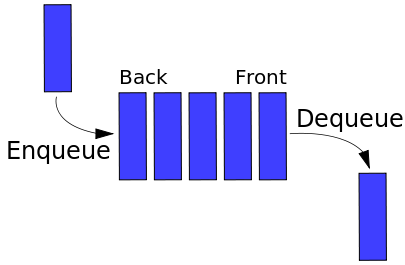
\includegraphics[height=3cm]{queue1.png}
\caption{队列的结构}
\end{figure}

下面的程序使用一个数组实现队列,为了减少空间的浪费,我们使数组的头和尾接在一起,形成一个环。这样做的好处是当DEQUEUE操作多次之后,我们可以利用已删除节点留下的空间。

\begin{figure}[htbp]
\centering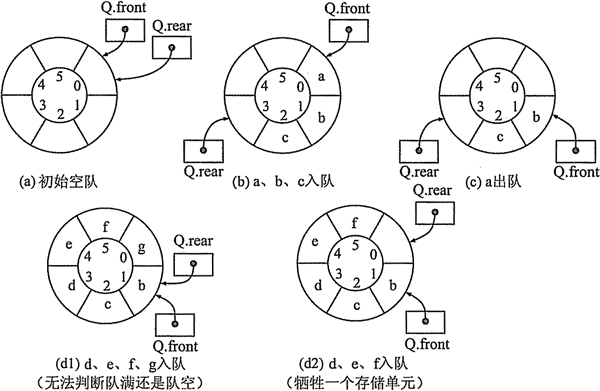
\includegraphics[height=7cm]{circlequeue.jpg}
\caption{循环队列的原理}
\end{figure}
\newpage

\begin{lstlisting}[language=C++]
/*
** A queue implemented with a static array.  The array size can
** be adjusted only by changing the #define and recompiling
** the module.
*/
#include "queue.h"
#include <stdio.h>
#include <assert.h>

#define	QUEUE_SIZE	100	/* Max # of values on the queue */
#define	ARRAY_SIZE	( QUEUE_SIZE + 1 )	/* Size of array */

/*
**	The array that holds the values on the queue, and pointers
**	to the front and rear of the queue.
*/
static	QUEUE_TYPE	queue[ ARRAY_SIZE ];
static	size_t		front = 1;
static	size_t		rear = 0;

/*
**	insert
*/
void
insert( QUEUE_TYPE value )
{
	assert( !is_full() );
	rear = ( rear + 1 ) % ARRAY_SIZE;
	queue[ rear ] = value;
}

/*
**	delete
*/
void
delete( void )
{
	assert( !is_empty() );
	front = ( front + 1 ) % ARRAY_SIZE;
}

/*
**	first
*/
QUEUE_TYPE first( void )
{
	assert( !is_empty() );
	return queue[ front ];
}

/*
**	is_empty
*/
int
is_empty( void )
{
	return ( rear + 1 ) % ARRAY_SIZE == front;
}

/*
**	is_full
*/
int
is_full( void )
{
	return ( rear + 2 ) % ARRAY_SIZE == front;
}
\end{lstlisting}

在学习了下面的内容之后,我们会有另一种队列的实现,代码也比较简单,读者可以自己实现。

\subsection{链表}

如果想对数组里的元素进行插入删除操作,那么每次操作将会付出很大的时间代价,这是不明智的。更好的办法是使用链表替代数组。

\subsubsection{单链表}
链表中最简单的一种是单向链表,它包含两个域,一个信息域和一个指针域。指针域指向列表中的下一个节点,而最后一个节点则指向一个空值。如图4所示,A指向B,我们称A为B的前驱,B为A的后继。

\begin{figure}[htbp]
\centering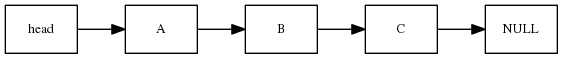
\includegraphics[height=1.2cm]{linklist1.png}
\caption{单链表的结构}
\end{figure}

一个单向链表的节点被分成两个部分。第一个部分保存或者显示关于节点的信息,第二个部分存储下一个节点的地址。单向链表只可向一个方向遍历。

\begin{figure}[htbp]
\centering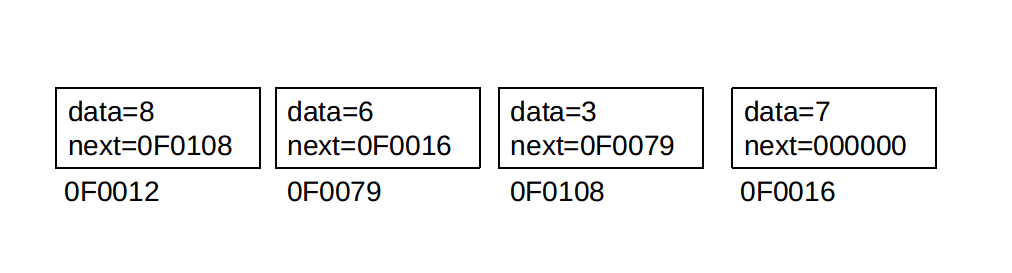
\includegraphics[height=3cm]{linkList4.png}
\caption{单链表的物理结构,$8\rightarrow 3\rightarrow 6\rightarrow 7$}
\end{figure}


链表最基本的结构是在每个节点保存数据和到下一个节点的地址,在最后一个节点保存一个特殊的结束标记,另外在一个固定的位置保存指向第一个节点的指针,有的时候也会同时储存指向最后一个节点的指针。\\
单链表的存储结构如下:

\begin{lstlisting}[language=C++]
typedef struct LNode{
    ElemType data;
    struct LNode *next;
}LNode, *LinkList;
\end{lstlisting}

为了操作方便,我们令单链表有一个头指针,它不存储任何数据,仅仅是一个空节点,并指向链表的第一个节点(如果有的话)。初始化一个链表时,只需要加入头结点即可。

\begin{lstlisting}[language=C++]
void InitList(LinkList *L)
{
    *L=(LinkList)malloc(sizeof(struct LNode));
    if(!*L)
        exit(OVERFLOW);
    (*L)->next=NULL;
}
\end{lstlisting}

链表的操作要点在于插入和删除,掌握了插入和删除,就相当于掌握了链表。

如果要删除一个节点,需要一个指向该节点和指向它的前驱节点的指针。

\begin{figure}[htbp]
\centering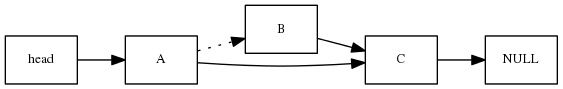
\includegraphics[height=1.7cm]{linklist2.png}
\caption{单链表的删除: 将$A\rightarrow B$链断开,指向$C$}
\end{figure}

\begin{lstlisting}[language=C++]
beforep->next = deletep->next;
free(deletep);
\end{lstlisting}


如果只知道需要删除的节点的指针$p$,可以使用下面的方式将其删除。但是需要保证$p\rightarrow next\neq NULL$才可以使用这种方式。当然,如果在实现时不考虑空节点和非空节点类型上的区别,就可以不需要这条保证了。美中不足的是,这样实际删除的不是$p$指向的节点而是它之后的节点,这也是数据结构考试时这么写不会得到分数的原因。
\begin{lstlisting}[language=C++]
*p = *p->next
//you should free one node here
\end{lstlisting}

如果要在节点p之后插入一个节点new\_ p,则只需要一个指向p的指针。

\begin{figure}[htbp]
\centering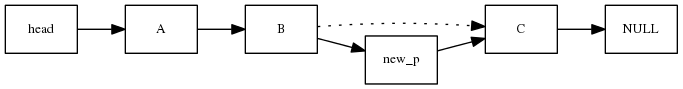
\includegraphics[height=1.6cm]{linklist3.png}
\caption{单链表的插入: $new\_p$ 指向$C$,再将$B\rightarrow C$断开,指向$new\_ p$}
\end{figure}

\begin{lstlisting}[language=C++]
new_p->next = p->next;
p->next = new_p;
\end{lstlisting}

下面给出部分参考代码代码。
\begin{lstlisting}[language=C++]
typedef	struct	NODE	{
	struct	NODE	*link;
	int		value;
} Node;

/*
** Insert into an ordered, singly linked list.  The arguments are
** a pointer to the first node in the list, and the value to
** insert.
*/
#include <stdlib.h>
#include <stdio.h>
#include "sll_node.h"

#define	FALSE	0
#define TRUE	1

int
sll_insert( register Node **linkp, int new_value )
{
	register Node	*current;
	register Node	*new;

	/*
	** Look for the right place by walking down the list
	** until we reach a node whose value is greater than
	** or equal to the new value.
	*/
	while( ( current = *linkp ) != NULL &&
	    current->value < new_value )
		linkp = &current->link;

	/*
	** Allocate a new node and store the new value into it.
	** In this event, we return FALSE.
	*/
	new = (Node *)malloc( sizeof( Node ) );
	if( new == NULL )
		return FALSE;
	new->value = new_value;

	/*
	** Insert the new node into the list, and return TRUE.
	*/
	new->link = current;
	*linkp = new;
	return TRUE;
}
\end{lstlisting}

以及比较通俗的版本。
\begin{lstlisting}[language=C++]
/*
** Insert into an ordered, singly linked list.  The arguments are
** a pointer to the first node in the list, and the value to
** insert.
*/
#include <stdlib.h>
#include <stdio.h>
#include "sll_node.h"

#define	FALSE	0
#define	TRUE	1

int
sll_insert( Node *current, int new_value )
{
	Node	*previous;
	Node	*new;

	/*
	** Look for the right place by walking down the list
	** until we reach a node whose value is greater than
	** or equal to the new value.
	*/
	while( current->value < new_value ){
		previous = current;
		current = current->link;
	}

	/*
	** Allocate a new node and store the new value into it.
	** In this event, we return FALSE.
	*/
	new = (Node *)malloc( sizeof( Node ) );
	if( new == NULL )
		return FALSE;
	new->value = new_value;

	/*
	** Insert the new node into the list, and return TRUE.
	*/
	new->link = current;
	previous->link = new;
	return TRUE;
}
\end{lstlisting}

\subsubsection{双链表}

与单链表不同的是,双链表增加了一个指向前驱的指针。插入和删除时,需要注意区分是否为最后一个节点。

\begin{figure}[htbp]
\centering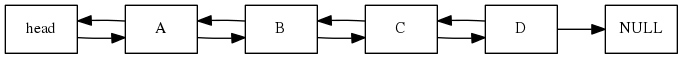
\includegraphics[height=1cm]{dlinklist.png}
\caption{双链表}
\end{figure}
\newpage
\begin{lstlisting}[language=C++]
typedef struct NODE {
	int data;
	struct NODE *left;
	struct NODE *right;
} Node;
\end{lstlisting}


将节点p删除的主要代码如下。除了这些,还要判断p是不是最后一个节点,因为最后一个节点是没有$p\rightarrow right\rightarrow left$的。不允许一段已经申请的内存没有指针指向它,在这种情况出现之前,需要将内存释放。\footnote{$free(p)$\ in C and $delete\ p$ in C++}
\begin{lstlisting}[language=C++]
p->left->right = p->right;
p->right->left = p->left;
\end{lstlisting}

如果还想将已经从链表中删除的p节点找回\footnote{感兴趣的同学可以参考文献\cite{knuth2000dancing}。} ,可以使用如下代码。
\begin{lstlisting}[language=C++]
p->left->right = p;
p->right->left = p;
\end{lstlisting}

如果要在p节点之后插入节点$new\_node$,同样需要判断p节点是不是最后一个节点,理由与之前一样。
\begin{lstlisting}[language=C++]
new_node->left = p;
new_node->right = p->right;
p->right->left = new_node;
p->right = new_node;
\end{lstlisting}
如果不想在每次删除或插入节点时都判断是否是最后一个节点,可以人为地加入一个空的尾节点,就像空的头结点一样。

\section{树形结构}

\subsection{二叉树}

二叉树是与链表类似的数据结构,不同于链表的是二叉树的每个节点有两个后继,分别称为左孩子和右孩子。每个节点至多只有一个前驱,称为父亲。

\begin{figure}[htbp]
\centering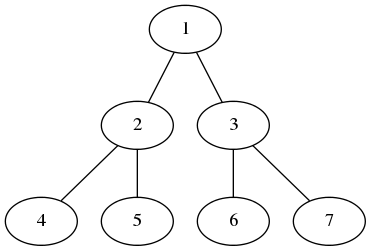
\includegraphics[height=6cm]{bt1.png}
\caption{二叉树}
\end{figure}

图9是一棵完全二叉树,除了使用链结构表示之外,还可以使用数组表示:节点$i$的左孩子标号为$2i$,右孩子标号为$2i+1$,它的父亲节点标号为$i/2$。

为了加深理解,我们讲解一种二叉树的应用。

\subsubsection*{二叉查找树}
二叉查找树(Binary Search Tree),也称有序二叉树(ordered binary tree),排序二叉树(sorted binary tree),是指一棵空树或者具有下列性质的二叉树:
\begin{enumerate}
\item 若任意节点的左子树不空,则左子树上所有结点的值均小于它的根结点的值;
\item 任意节点的右子树不空,则右子树上所有结点的值均大于它的根结点的值;
\item 任意节点的左、右子树也分别为二叉查找树;
\item 没有键值相等的节点。
\end{enumerate}

\begin{figure}[htbp]
\centering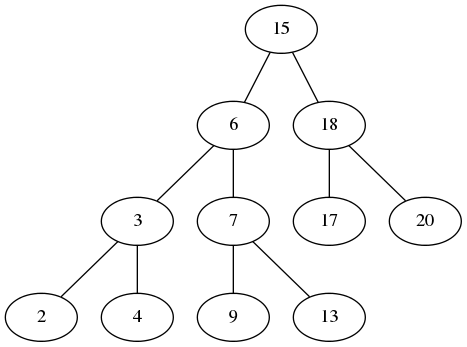
\includegraphics[height=6cm]{bt2.png}
\caption{二叉查找树}
\end{figure}

二叉查找树相比于其他数据结构的优势在于查找、插入的时间复杂度较低。为O(log n)。二叉查找树是基础性数据结构,用于构建更为抽象的数据结构,如集合、multiset、关联数组等。

二叉查找树的查找过程和次优二叉树类似,通常采取二叉链表作为二叉查找树的存储结构。中序遍历二叉查找树可得到一个关键字的有序序列,一个无序序列可以通过构造一棵二叉查找树变成一个有序序列,构造树的过程即为对无序序列进行查找的过程。每次插入的新的结点都是二叉查找树上新的叶子结点,在进行插入操作时,不必移动其它结点,只需改动某个结点的指针,由空变为非空即可。搜索,插入,删除的复杂度等于树高,期望O(log n),最坏O(n)(数列有序,树退化成线性表).

虽然二叉查找树的最坏效率是$O(n)$,但它支持动态查询,且有很多改进版的二叉查找树可以使树高为$O(logn)$,如SBT,AVL,红黑树等.故不失为一种好的动态查找方法.

在二叉查找树b中查找x的过程为:
\begin{enumerate}
\item 若b是空树,则搜索失败,否则:
\item 若x等于b的根节点的数据域之值,则查找成功;否则:
\item 若x小于b的根节点的数据域之值,则搜索左子树;否则:
\item 查找右子树。
\end{enumerate}


向一个二叉查找树b中插入一个节点s的算法,过程为:
\begin{enumerate}
\item 若b是空树,则将s所指结点作为根节点插入,否则:
\item 若$s\rightarrow data$等于b的根节点的数据域之值,则返回,否则:
\item 若$s\rightarrow data$小于b的根节点的数据域之值,则把s所指节点插入到左子树中,否则:
\item 把s所指节点插入到右子树中。
\end{enumerate}

在二叉查找树删去一个结点,分三种情况讨论:
\begin{enumerate}
\item 若*p结点为叶子结点,即PL(左子树)和PR(右子树)均为空树。由于删去叶子结点不破坏整棵树的结构,则只需修改其双亲结点的指针即可。
\item 若*p结点只有左子树PL或右子树PR,此时只要令PL或PR直接成为其双亲结点*f的左子树(当*p是左子树)或右子树(当*p是右子树)即可,作此修改也不破坏二叉查找树的特性。
\item 若*p结点的左子树和右子树均不空。在删去*p之后,为保持其它元素之间的相对位置不变,可按中序遍历保持有序进行调整,可以有两种做法:其一是令*p的左子树为*f的左/右(依*p是*f的左子树还是右子树而定)子树,*s为*p左子树的最右下的结点,而*p的右子树为*s的右子树;其二是令*p的直接前驱(in-order predecessor)或直接后继(in-order successor)替代*p,然后再从二叉查找树中删去它的直接前驱(或直接后继)。
\end{enumerate}

\paragraph{二叉树的遍历} 一棵非空的二叉树由根结点及左、右子树这三个基本部分组成。因此,在任一给定结点上,可以按某种次序执行三个操作:
\begin{enumerate}
\item 访问结点本身(N), 
\item 遍历该结点的左子树(L), 
\item 遍历该结点的右子树(R)。
\end{enumerate}

以上三种操作有六种执行次序:
NLR、LNR、LRN、NRL、RNL、RLN。
注意:
前三种次序与后三种次序对称,故只讨论先左后右的前三种次序。\\
① NLR:前序遍历(PreorderTraversal亦称先序遍历)\\
	——访问根结点的操作发生在遍历其左右子树之前。\\
② LNR:中序遍历(InorderTraversal)\\
	——访问根结点的操作发生在遍历其左右子树之中。\\
③ LRN:后序遍历(PostorderTraversal)\\
	——访问根结点的操作发生在遍历其左右子树之后。


\paragraph{二叉查找树性能分析}%
每个结点的$C_i$为该结点的层次数。最坏情况下,当先后插入的关键字有序时,构成的二叉查找树蜕变为单支树,树的深度为$n$,其平均查找长度为$\frac{n+1}{2}$(和顺序查找相同),最好的情况是二叉查找树的形态和折半查找的判定树相同,其平均查找长度和$\log_2(n)$成正比($O(\log_2(n))$)。

\subsection{并查集}

在计算机科学中,并查集是一种树型的数据结构,其保持着用于处理一些不相交集合(Disjoint Sets)的合并及查询问题。有一个联合--查找算法(union-find algorithm)定义了两个操作用于此数据结构:



\begin{description}
  \item[Find:] 确定元素属于哪一个子集。它可以被用来确定两个元素是否属于同一子集。
  \item[Union:] 将两个子集合并成同一个集合。
\end{description}

因为它支持这两种操作,一个不相交集也常被称为联合-查找数据结构(union-find data structure)或合并-查找集合(merge-find set)。其他的重要方法,MakeSet,用于建立单元素集合。有了这些方法,许多经典的划分问题可以被解决。

并查集森林是一种将每一个集合以树表示的数据结构,其中每一个节点保存着到它的父节点的引用。这个数据结构最早由Bernard A. Galler和Michael J. Fischer于1964年提出,\cite{Galler} 但是经过了数年才完成了精确的分析。

在并查集森林中,每个集合的代表即是集合的根节点。“查找”根据其父节点的引用向根行进直到到底树根。“联合”将两棵树合并到一起,这通过将一棵树的根连接到另一棵树的根。实现这样操作的一种方法是:


\begin{lstlisting}[language=pascal]
 function MakeSet(x)
     x.parent := x

 function Find(x)
     if x.parent == x
        return x
     else
        return Find(x.parent)

 function Union(x, y)
     xRoot := Find(x)
     yRoot := Find(y)
     xRoot.parent := yRoot
\end{lstlisting}

这是并查集森林的最基础的表示方法,这个方法不会比链表法好,这是因为创建的树可能会严重不平衡;然而,可以用两种办法优化。

第一种方法,称为“按秩合并”,即总是将更小的树连接至更大的树上。因为影响运行时间的是树的深度,更小的树添加到更深的树的根上将不会增加秩除非它们的秩相同。在这个算法中,术语“秩”替代了“深度”,因为同时应用了路径压缩时(见下文)秩将不会与高度相同。单元素的树的秩定义为0,当两棵秩同为r的树联合时,它们的秩r+1。只使用这个方法将时最坏的运行时间提高至每个MakeSet、Union或Find操作$O(\log n)$。优化后的MakeSet和Union伪代码:

\begin{lstlisting}[language=pascal]
 function MakeSet(x)
     x.parent := x
     x.rank   := 0

 function Union(x, y)
     xRoot := Find(x)
     yRoot := Find(y)
     if xRoot == yRoot
         return
     if xRoot.rank < yRoot.rank
         xRoot.parent := yRoot
     else if xRoot.rank > yRoot.rank
         yRoot.parent := xRoot
     else
         yRoot.parent := xRoot
         xRoot.rank := xRoot.rank + 1
\end{lstlisting}

第二个优化,称为“路径压缩”,是一种在执行“查找”时扁平化树结构的方法。关键在于在路径上的每个节点都可以直接连接到根上;他们都有同样的表示方法。为了达到这样的效果,Find递归地经过树,改变每一个节点的引用到根节点。得到的树将更加扁平,为以后直接或者间接引用节点的操作加速。这儿是Find:
\begin{lstlisting}[language=pascal]
 function Find(x)
     if x.parent != x
        x.parent := Find(x.parent)
     return x.parent
\end{lstlisting}

Michael Fredman和Saks在1989年解释了$\Omega(\alpha(n))$的平均时间内可以获得任何并查集。

下面给出完整的C++语言代码。

\begin{lstlisting}[language=C++]
int par[MAX_N];
int rank[MAX_N];

void init(int n) {
    for(int i = 0; i < n; i++) {
        par[i] = i;
        rank[i] = 0;
    }
}

int find(int x) {
    if(par[x] == x) {
        return x;
    } else {
        return par[x] = find(par[x]);
    }
}

void unite(int x, int y) {
    x = find(x);
    y = find(y);
    if(x == y) return ;
    if(rank[x] < rank[y]) {
        par[x] = y;
    } else {
        par[y] = x;
        if(rank[x] == rank[y]) rank[x]++;
    }
}

bool same(int x, int y) {
    return find(x) == find(y);
}
\end{lstlisting}

\subsection{堆}

堆(英语:heap)亦被称为:优先队列(英语:priority queue),是计算机科学中一类特殊的数据结构的统称。堆通常是一个可以被看做一棵树的数组对象。在队列中,调度程序反复提取队列中第一个作业并运行,因而实际情况中某些时间较短的任务将等待很长时间才能结束,或者某些不短小,但具有重要性的作业,同样应当具有优先权。堆即为解决此类问题设计的一种数据结构。\cite{shaffer}

\paragraph{逻辑定义}
n个元素序列$\{k_1,k_2...k_i...k_n\}$,当且仅当满足下列关系时称之为堆:

$(k_i <= k_{2i},k_i <= k_{2i+1})$或者$(k_i >= k_{2i},ki >= k_{2i+1}), (i = 1,2,3,4...n/2)$

堆的实现通过构造二叉堆(binary heap),实为二叉树的一种;由于其应用的普遍性,当不加限定时,均指该数据结构的这种实现。这种数据结构具有以下性质。
\begin{itemize}
  \item 任意节点小于它的所有后裔,最小元在堆的根上(堆序性)。
  \item 堆总是一棵完全树。
\end{itemize}

将根节点最大的堆叫做最大堆或大根堆,根节点最小的堆叫做最小堆或小根堆。常见的堆有二叉堆、斐波那契堆等。

为将元素X插入堆中,找到空闲位置,建立一个空穴,若满足堆序性(英文:heap order),则插入完成;否则将父节点元素装入空穴,删除该父节点元素,完成空穴上移。直至满足堆序性。这种策略叫做上滤(percolate up)。\cite{shaffer}

DeleteMin,删除最小元,即二叉树的根或父节点。删除该节点元素后,队列最后一个元素必须移动到堆得某个位置,使得堆仍然满足堆序性质。这种向下替换元素的过程叫作下滤。

下面给出示例代码。push向堆中插入一个元素,pop将堆顶元素删除并返回。

\begin{lstlisting}[language=C++]
int heap[MAX_N], sz = 0;
void push(int x) {
    int i = sz++;
    while(i > 0) {
        int p = (i - 1) / 2;
        if(heap[p] <= x) break;
        heap[i] = heap[p];
        i = p;
    }
    heap[i] = x;
}
int pop() {
    int ret = heap[0];
    int x = heap[--sz];
    int i = 0;
    while(i * 2 + 1 < sz) {
        int a = i * 2 + 1, b = i * 2 + 2;
        if(b < sz && heap[b] < heap[a]) a = b;
        if(heap[a] >= x) break;
        heap[i] = heap[a];
        i = a;
    }
    heap[i] = x;
    return ret;
}
\end{lstlisting}


\section{初识有限状态自动机}
\subsection{简单介绍}
这里我们仅仅设计自动机的轮廓,更高深的内容可以查阅文献\cite{rich2008automata}。

我们用仅包含两个符号''a''和''b''来说明自动机的轮廓。图9中的自动机会接受''ab''这样的输入,但会拒绝其他任何输入。
自动机一开始处于start状态。如果输入的第一个字符是''a'',它将前进到状态2,如果是''b'',则前进 到状态3.在状态2,如果输入的第二个字符是''b'',自动机则前进到最终状态,如果是''a'',则前进到状态3。在最终状态如果继续输入,自动机就会离开最终状态,到达没有出口的状态3。因此,这个自动机能够接受的输入只有''ab''。如果自动机接受到输入的最后一个字符,并且停留在最终状态,那么它就是被接受的。除此之外,全部被拒绝。

\begin{figure}[htbp]
\centering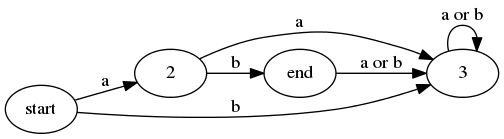
\includegraphics[height=3cm]{auto.png}
\caption{接受"ab"输入的有限状态自动机}
\end{figure}

我们也可以设计能接受任意长度字符串的自动机。图10的自动机会接受形如''ab''、''abab''、''ababab''的字符串。

\begin{figure}[htbp]
\centering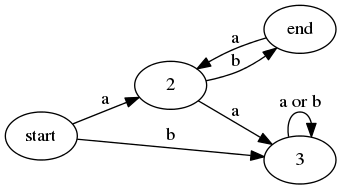
\includegraphics[height=3.6cm]{auto2.png}
\caption{接受''ab''、''abab''、''ababab'' $\cdots$ 输入的有限状态自动机}
\end{figure}
\subsection{字符串匹配自动机}
如果我们根据一个字符串按照下面的算法构造,就会得到一种非常有用的自动机。
\begin{enumerate}
\item 每个节点有两条边,分别为$if$边和$next$边,$if$边有一个值。
\item 令$start$为初始状态节点,$p$和$q$为指向节点的指针。令$start\rightarrow next$指向$start$,输入一个字符$c$,建立新节点$new\_ node$,令$start\rightarrow if$边的值为$c$,指向$new\_ node$,$new\_ node\rightarrow next$指向$start$。令$p$指向$new\_ node$,$q$指向$start$。
\item 按照输入顺序建立新节点,并令节点的$if$边顺次连接各节点,边的值为对应字符的值,最后的检点标记为$end$,令$end\rightarrow if=NULL$,$end\rightarrow next=end$。
\item 若$p\neq end$执行操作5;否则结束。
\item 
\begin{enumerate}
\item 如果$q==start$或$p\rightarrow if$的值和$q\rightarrow if$的值相等,则$p$指向$p\rightarrow if$指向的节点,$q$指向$q\rightarrow if$指向的节点,$p\rightarrow next$指向$q$
\item 否则令$q$指向$q\rightarrow next$
\item 执行操作4。
\end{enumerate}
\end{enumerate}

\begin{figure}[htbp]
\centering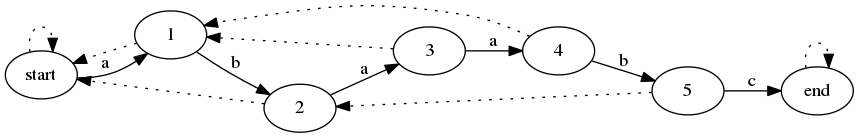
\includegraphics[height=2cm]{auto3.png}
\caption{由''abaabc''生成的自动机,该自动机接受包含子字符串''abaabc''的所有字符串}
\end{figure}

更详细的内容会在讲字符串的时候接触到,不再赘述。

\newpage
\nocite{*}
\bibliographystyle{plain}
\bibliography{bibfile}


\end{CJK}

\end{document}
